\subsection{Previous Work}

% \begin{itemize}
%     \item Introduce previous papers \citepsixth{p6Alvarez2018,Alvarez2018a,Baldwin2017,Baldwin2017a}
%     \item Discuss the approach again, explicitly stating that it is an extension and how it extends \citepsixth{p6alvarez2019empowering}
%     \item Besides the experiments and user study, we also added two new dimensions (leniency and inner\_similarity) --> Perhaps this should be in another part. Added to Section III
%     \item Introduce papers that evaluate content generators \citepsixth{p6Smith:2010:Expressive-range,Cook2016-danesh,Cook2019:ParameterBasedEvaluation}
% \end{itemize}{}

% \subsubsection{Dungeons}
% For more than 40 years, \emph{dungeons} have frequently been the setting for digital games and provided players with entertainment and excitement in particularly computer role-playing games (CRPGs) and adventure games. It seems that dungeons, as game settings, are as popular as ever, and shows no signs of going away~\citepsixth{p6totten2017}. We can trace the first digital dungeons to the PLATO system back in 1975~\citepsixth{p6barton08dad,brewer2016b} with games called ``\emph{pedit5}''~\citepsixth{p6pedit5} and ``\emph{moria}''. Even though the layout of the dungeon in ``\emph{pedit5}'' was a fixed design, the game contained randomly generated encounters and rewards, making it a predecessor to the more commonly known \emph{Rogue}~\citepsixth{p6michael_toy_1980} which provides the player with a new layout of the dungeon with every restart. However, prior to \emph{Rogue}, the game \emph{Beneath Apple Manor}~\citepsixth{p6applemanor} made for the Apple contained a level generator which gave the player the possibility to replay the game with a different layout when starting the game. This feature of dungeons as ``randomized environments'' is the key element in so called Dungeon Hack games~\citepsixth{p6batemanboon}. 

% With regards to CRPGs and adventure games, it should be noted that they share the mechanisms of adventure and exploration whereas combat is more common in CRPG~\citepsixth{p6rollings-adams}. Adventure games, on the other hand, more often contain puzzle solving as a mechanism. It is perhaps not that strange that dungeons are a popular setting for games in these genres, since they provide the following design elements: levels (several levels are needed with diverse layout and difficulty), collectibles (loot), boss fights, locked door and key (you need to find the key to open the door), wildcard enemies (placement, type and strength), monster generators (new monsters are generated until this mechanism is destroyed), and finally, exits and warps (which acts as transitions to other parts indicating progress in the game)~\citepsixth{p6rollings-adams}. 

\subsubsection{Map-Elites for illuminating search spaces}

Quality-diversity algorithms are algorithms which search a %space of solutions 
solution space, not just for the single best solution, but for a set of diverse solutions which are high performing. MAP-Elites maintains of map of good solutions~\citepsixth{p6Mouret2015} and is a well-known quality-diversity algorithm%~\citepsixth{p6fontaine2019covariance}
. The map is divided into a number of cells according to one or more feature dimensions. In each cell, a single solution is kept. At every update, an offspring is generated based on one or more existing solutions. That offspring     is then assigned to a cell based on its feature dimensions, which might or might not be the same as the cell(s) its parent(s) occupy. %If the new offspring has a higher fitness than the existing solution in that cell, it replaces the cell.
If the new offspring has a higher fitness than the existing solution in that cell, it replaces the previous item in the cell. This process results in a map of solutions where each cell contains the best found solution for those particular feature dimensions.

\subsubsection{Evaluation of Procedural Content Generators}
%In essence, any venture that applies PCG approaches strive to automate the process of creating game content. 
Shaker, et al.~\citepsixth{p6shaker_procedural_2016}, argues that ultimately the evaluation of content generators is to verify that they fulfil their design goals. In order to be able to understand or modify a generator it is important to visualize its content space. However, it is seldom enough to look at a single individual piece of content, but rather it is vital to examine the frequency the different features appear, or the amount of variety the features demonstrate. Previous attempts of doing this are termed expressivity measures~\citepsixth{p6Smith:2010:Expressive-range,p6Summerville2018-ExpresiveRange} and have, for instance, explored difficulty measures~\citepsixth{p6Horn2014-comparativePCG}. Other approaches incorporate tool assisted parameter exploration due to its effect on the content space~\citepsixth{p6Cook2016-danesh,p6Cook2019:ParameterBasedEvaluation}.

%that fulfil a set of criteria for the content product. 
%If we for the moment disregard more exact definitions to allow for a more general and principal discussion, game content must be usable in its user-context. For MI: design-time, runtime?...

\subsubsection{Evolving Dungeons as a Whole, Room by Room}

% \begin{figure}[t]
% \centerline{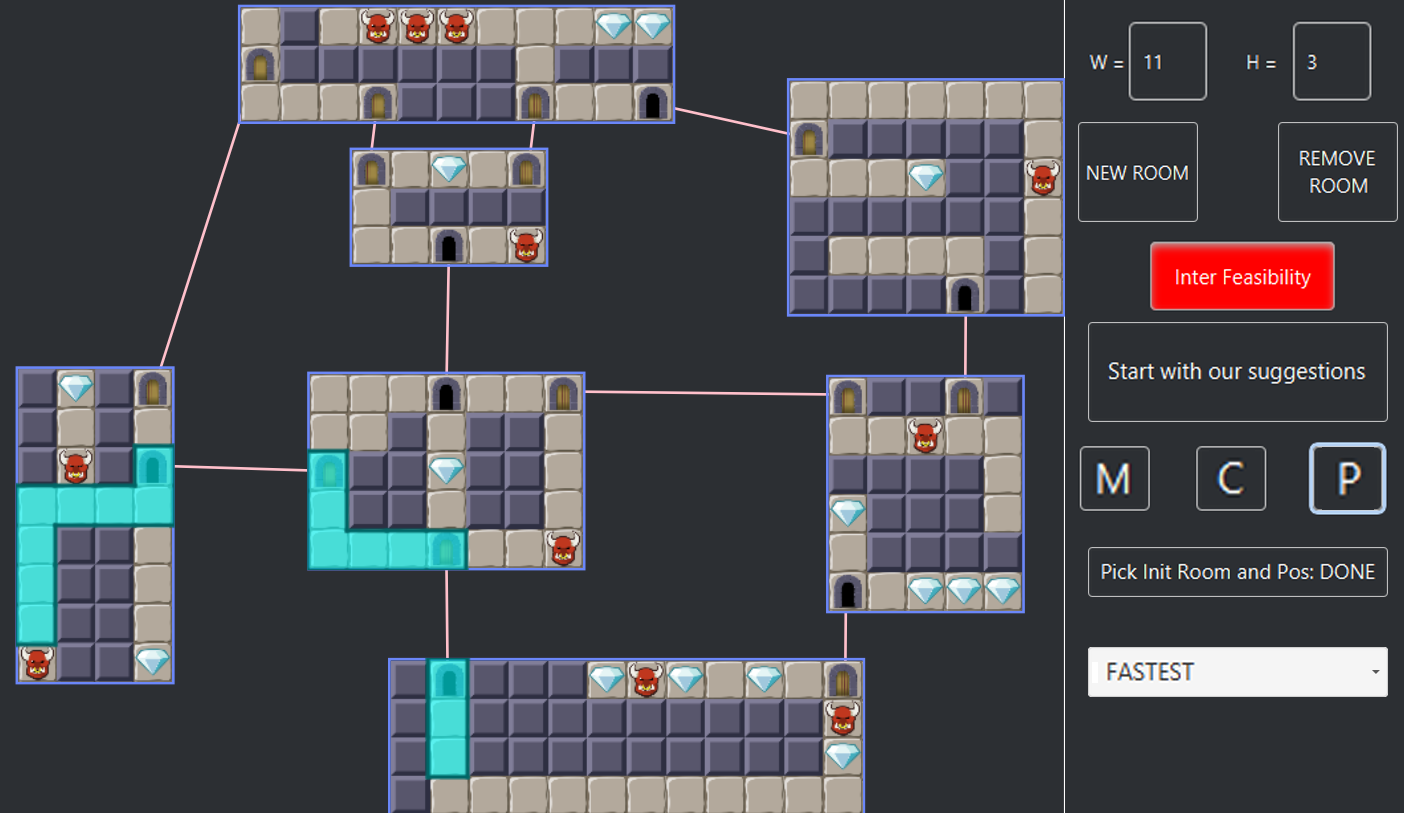
\includegraphics[width=9cm]{figures/figure2.png}}
% \caption{Screenshot of the dungeon editor screen in EDD, displaying a sample dungeon composed by seven rooms. The shortest path between two given tiles is highlighted in blue. The right pane contains all options for editing the dungeon. "M", "C", and "P" stand for "Move rooms", "Connect rooms", and "calculate Path".}
% \label{figs:dungeonscreen}
% \end{figure}

EDD is a MI-CC tool that allows a human designer to create a 2D dungeon and the rooms it is composed of%(\Cref{figs:basecomponents}.a)
. The designer is able to manually edit both the dungeon by placing and removing rooms, and the individual rooms by  editing the tiles %(\Cref{figs:basecomponents}.b) 
that each room consists of. EDD's underlying evolutionary algorithm provides procedurally generated suggestions, and is driven through the use of game design micro- and meso- patterns%(\Cref{figs:basecomponents}.c and \Cref{figs:basecomponents}.d)
. A detailed description of all EDD's features, including the use of game design patterns, can be found in~\citepsixth{p6Baldwin2017a,p6Baldwin2017,p6Alvarez2018,p6Alvarez2018a}, where \citepsixth{p6Alvarez2018,p6Baldwin2017} analyze and discuss the mixed-initiative system in EDD and \citepsixth{p6Baldwin2017a,p6Alvarez2018a} focus on the procedural content generator.

% \begin{figure*}[t]
% \centerline{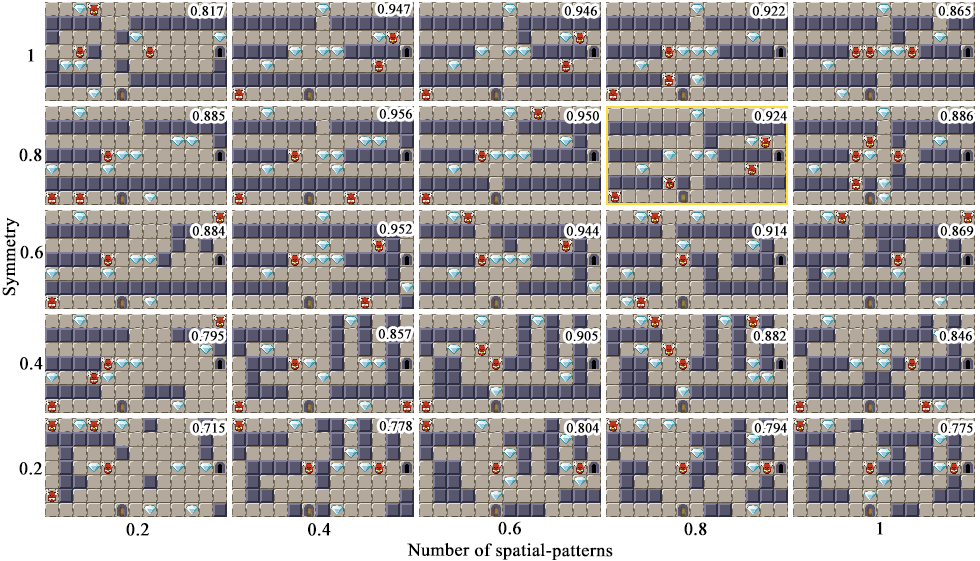
\includegraphics[width=11cm]{figures/figure3.jpg}}
% \caption{The room editor screen in EDD. The left pane contains all the options for manually editing the room displayed at the center-left of the screen. The right section displays the procedurally generated suggestions.}
% \label{figs:roomscreen}
% \end{figure*}

\begin{figure}[t]
\centerline{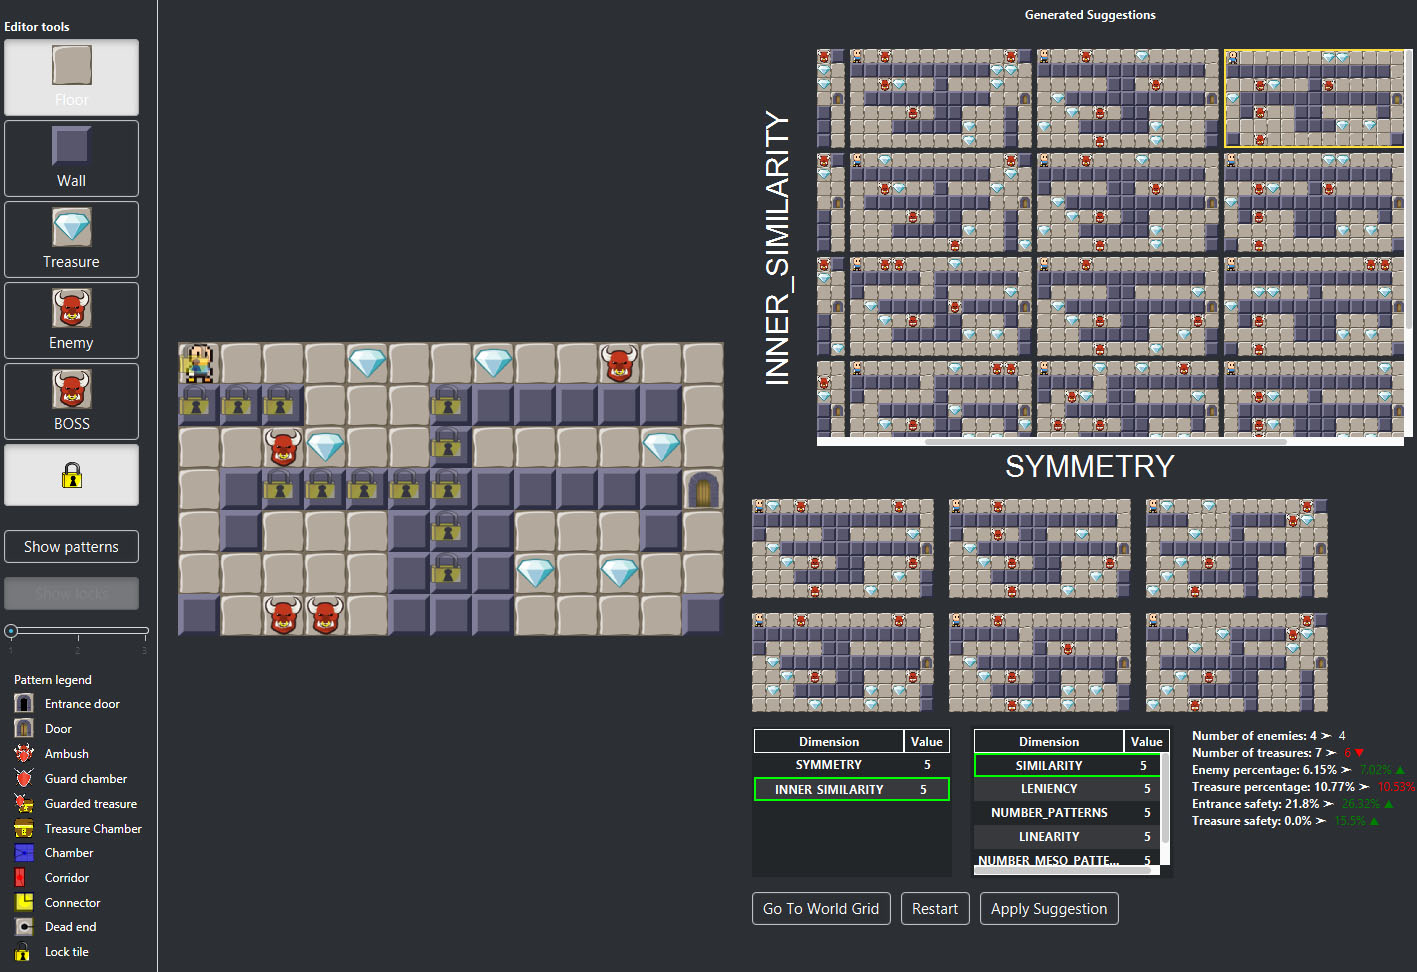
\includegraphics[width=0.8\textwidth]{figures/figure1.png}}
\caption{The room editor screen in EDD. The left pane contains all the options for manually editing the room displayed at the center-left of the screen. The right section displays the procedurally generated suggestions.}
\label{figs:roomscreen}
\end{figure}

In this section we present the latest version of EDD\footnote{Available for download at \url{https://github.com/mau-games/eddy}}, which includes significant improvements based on the outcomes from the qualitative analysis discussed in~\citepsixth{p6Alvarez2018}. The dungeon is now represented as a graph of interconnected rooms of any given size between $3\times3$ and $20\times20$ tiles. The smallest allowed dungeon is composed by two rooms with one connection to each other. Rooms and connections can now be added and removed at any time. Connections are marked with door tiles.

% perform the following new actions: 

% \begin{itemize}
% \item adding and removing rooms to the dungeon.
% \item connecting any pair of rooms by adding a new bi-directional connection to the graph. Rooms interconnect from and to passable border tiles (self-loops are not allowed). Both ends are marked with a door tile %(\Cref{figs:basecomponents}.b)
% . Connections and rooms can be removed at any time, and their associated doors removed with them.% Removing a room also removes its connections.
% \item calculating paths between any pair of passable tiles located in any connected room. Paths are automatically calculated according to \textit{fastest}, \textit{most treasures}, \textit{most danger}, and \textit{less danger} paths.
% \end{itemize}


% \begin{itemize}
% \item adding disconnected rooms to the dungeon. Rooms may also be removed at any time.
% \item connecting any pair of rooms by adding a new bi-directional connection to the graph. Rooms interconnect from and to passable border tiles (self-loops are not allowed). Both ends are marked with a door tile (\Cref{figs:basecomponents}.b). A single border tile can only hold one connection, implying that a room can have as many connections as passable border tiles. Connections and rooms can be removed at any time, and their associated doors removed with them.% Removing a room also removes its connections.
% \item calculating paths between any pair of passable tiles located in any connected room. Paths are automatically calculated according to one of the following heuristics: \textit{fastest} returns the shortest path, \textit{rewarding} returns the path that traverses the highest number of treasure tiles, \textit{less danger} provides a path with the fewest number of enemies, whereas \textit{more danger} does the opposite. 
% \end{itemize}

The designer marks one room as the \textit{initial room} for feasibility calculation: a dungeon is feasible when there is at least one path between the \textit{initial room} and any other passable tile in the dungeon. Rooms and doors that are unreachable from the \textit{initial room} are highlighted in red, so that they can be easily identified by the designer.

% The designer is required to select one of the added rooms as the \textit{initial room}, which is the first room the player meets when entering the dungeon. This selection can be modified unlimited times. The \textit{initial room} is used by EDD to calculate the feasibility of the dungeon. A dungeon is considered feasible when there is at least one path between the \textit{initial room} and any other passable tile in every room. Rooms and doors that are unreachable from the \textit{initial room} are highlighted in red, so that they can be easily identified by the designer. This feasibility constraint ensures that all passable tiles are accessible, avoiding the possibility of accidentally creating unreachable areas.  

% \paragraph{The mixed-initiative workflow in EDD}

The starting screen in EDD is the dungeon editor screen%, shown in \Cref{figs:dungeonscreen}
. Every new room is empty (composed solely of floor tiles) when created and is placed detached from the dungeon graph. After manually connecting the room to the dungeon with at least one connection, the designer has the option to populate the room using the room editor screen (\Cref{figs:roomscreen}). This screen can be reached by either double-clicking on the room or by clicking on the "Start with our suggestions" button, which will present six procedurally generated suggestions to the designer to start editing from. 

% The starting screen in EDD is the dungeon editor screen%, shown in \Cref{figs:dungeonscreen}
% . Every new room is empty (composed solely of floor tiles) when created and is placed detached from the dungeon graph. After manually connecting the room to the dungeon with at least one connection, the designer has the option to populate the room using the room editor screen (\Cref{figs:roomscreen}). This screen can be reached in two different ways:

% \begin{enumerate}
% \item directly: by double-clicking or zooming in (by using the mouse wheel or by pinching on the touchpad) on the room. 
% \item indirectly: by clicking on the "Start with our suggestions" button% on the right pane (\Cref{figs:dungeonscreen})
% , six procedurally generated suggestions are displayed on a separate screen. The selected suggestion is then opened in the room editor screen. 
% \end{enumerate}

\Cref{figs:roomscreen} shows the room editor screen displaying a sample room with the dimensions $7\times13$ tiles. The left pane lists all the available options for manually editing the room by brush painting with one of the available tile types (floor, wall, treasure, or enemy) and one of the two brush sizes (single tile and five-tile cross shape). Control-clicking allows the designer to bucket paint all adjacent tiles of the same type. Brush painting with the lock button on preserves selected tiles in all the procedurally generated suggestions. A detailed description of all the options in this pane is included in~\citepsixth{p6Alvarez2018,p6Alvarez2018a}.

The right side of the screen displays the procedurally generated suggestions, by means of the Interactive Constrained MAP-Elites (IC MAP-Elites) genetic algorithm (see \Cref{section:3}). %The "Generate/Stop Suggestions" button at the bottom toggles this algorithm on and off. 
When the designer accesses the room editor screen, IC MAP-Elites starts and continuously populates the suggestions pane with elites. The evolutionary process is fed with the manually edited room (i.e. target room), so that every change in the room affects the generated suggestions. By clicking on "Apply Suggestion", the manually edited room is replaced by the selected suggestion, thus affecting the upcoming procedural suggestions. "Restart" restarts evolution, and "Go To World Grid" takes the user back to the dungeon editor screen.